% Computational-to-neural functional correspondence (ANALOGY, not implementation).
% Compile: pdflatex fig10_neuromap.tex
\documentclass[border=6pt]{standalone}
\usepackage{amsmath,amssymb}
\usepackage{tikz}
\usetikzlibrary{arrows.meta,positioning,fit,backgrounds,calc}
\begin{document}
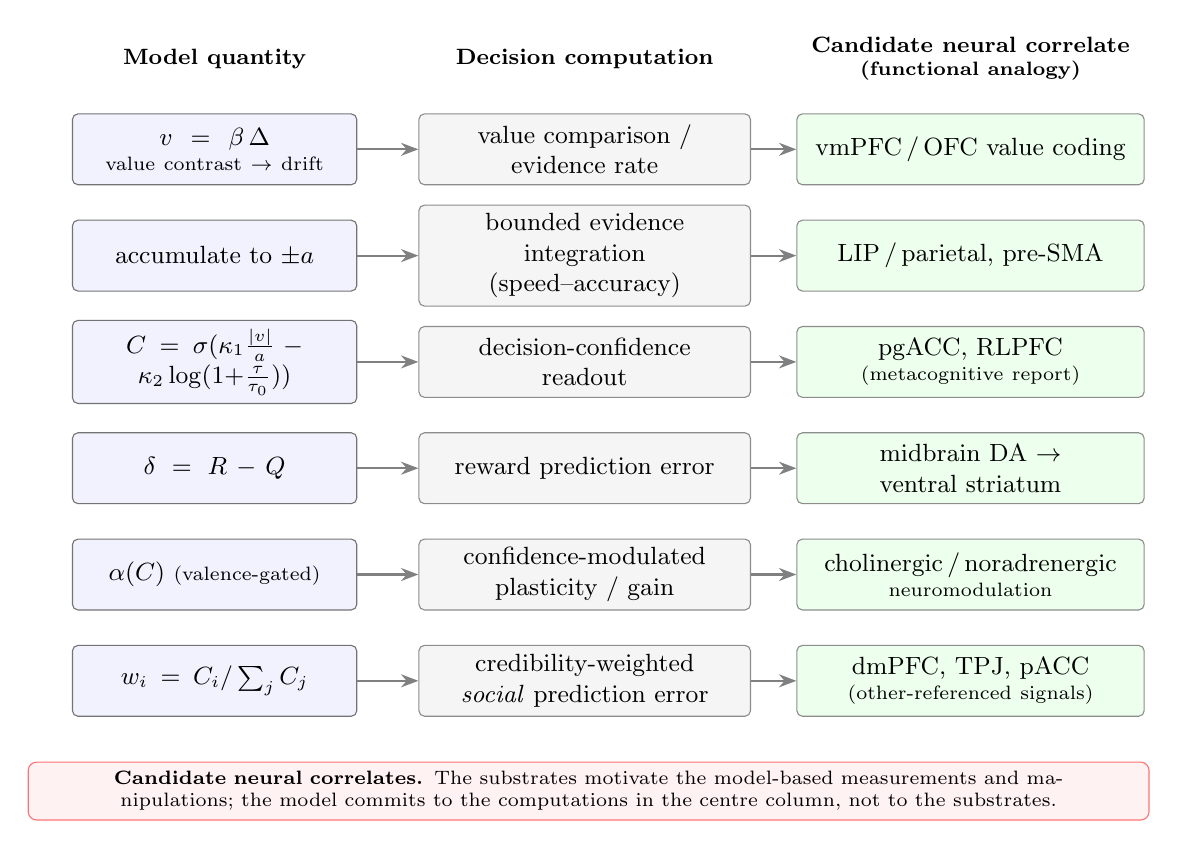
\begin{tikzpicture}[
  font=\small,>={Stealth[length=2.2mm]},
  mq/.style={draw=black!55,rounded corners=2pt,fill=blue!5,align=center,
             minimum height=9mm,text width=34mm,inner sep=3pt},
  cp/.style={draw=black!45,rounded corners=2pt,fill=black!4,align=center,
             minimum height=9mm,text width=40mm,inner sep=3pt},
  ns/.style={draw=black!45,rounded corners=2pt,fill=green!7,align=center,
             minimum height=9mm,text width=42mm,inner sep=3pt},
  hd/.style={font=\footnotesize\bfseries,align=center},
  ar/.style={->,thick,black!50},
]
% column headers
\node[hd] at (0,1.15)  {Model quantity};
\node[hd] at (4.7,1.15){Decision computation};
\node[hd] at (9.6,1.15){Candidate neural correlate\\[-1pt]\scriptsize(functional analogy)};

\def\yA{0.0}\def\yB{-1.35}\def\yC{-2.70}\def\yD{-4.05}\def\yE{-5.40}\def\yF{-6.75}

% row 1 -- value / drift
\node[mq] (m1) at (0,\yA) {$v=\beta\,\Delta$\\[-2pt]\scriptsize value contrast $\to$ drift};
\node[cp] (c1) at (4.7,\yA){value comparison /\\evidence rate};
\node[ns] (n1) at (9.6,\yA){vmPFC\,/\,OFC value coding};
% row 2 -- accumulation
\node[mq] (m2) at (0,\yB) {accumulate to $\pm a$};
\node[cp] (c2) at (4.7,\yB){bounded evidence\\integration (speed--accuracy)};
\node[ns] (n2) at (9.6,\yB){LIP\,/\,parietal, pre-SMA};
% row 3 -- confidence
\node[mq] (m3) at (0,\yC) {$C=\sigma(\kappa_1\tfrac{|v|}{a}-\kappa_2\log(1{+}\tfrac{\tau}{\tau_0}))$};
\node[cp] (c3) at (4.7,\yC){decision-confidence\\readout};
\node[ns] (n3) at (9.6,\yC){pgACC, RLPFC\\[-2pt]\scriptsize (metacognitive report)};
% row 4 -- reward PE
\node[mq] (m4) at (0,\yD) {$\delta=R-Q$};
\node[cp] (c4) at (4.7,\yD){reward prediction error};
\node[ns] (n4) at (9.6,\yD){midbrain DA $\to$ ventral striatum};
% row 5 -- gain
\node[mq] (m5) at (0,\yE) {$\alpha(C)$ \scriptsize(valence-gated)};
\node[cp] (c5) at (4.7,\yE){confidence-modulated\\plasticity / gain};
\node[ns] (n5) at (9.6,\yE){cholinergic\,/\,noradrenergic\\[-2pt]\scriptsize neuromodulation};
% row 6 -- social credibility
\node[mq] (m6) at (0,\yF) {$w_i=C_i/\textstyle\sum_j C_j$};
\node[cp] (c6) at (4.7,\yF){credibility-weighted\\\emph{social} prediction error};
\node[ns] (n6) at (9.6,\yF){dmPFC, TPJ, pACC\\[-2pt]\scriptsize (other-referenced signals)};

\foreach \i in {1,...,6}{\draw[ar] (m\i) -- (c\i); \draw[ar] (c\i) -- (n\i);}

% caveat banner
\node[draw=red!55,rounded corners=3pt,fill=red!5,text width=140mm,align=center,
      font=\scriptsize] at (4.75,-8.15)
  {\textbf{Candidate neural correlates.} The substrates motivate the model-based
   measurements and manipulations; the model commits to the computations in the
   centre column, not to the substrates.};
\end{tikzpicture}
\end{document}
